\begin{figure}[!ht]
    \centering
    \begin{subfigure}{1\linewidth}
        \centering
        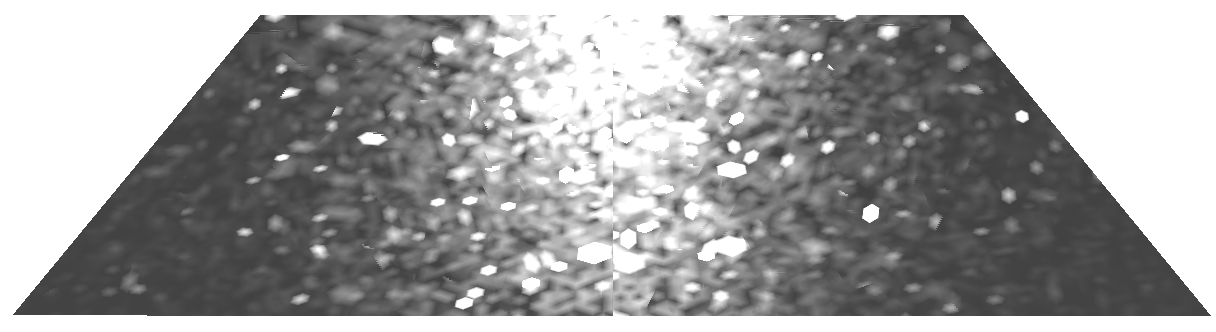
\includegraphics[width=0.5\linewidth]{artifact/linearsurface.png}
        \caption{Artifacts visible at high screen-space scale.}
    \end{subfigure}
    \begin{subfigure}{1\linewidth}
        \centering
        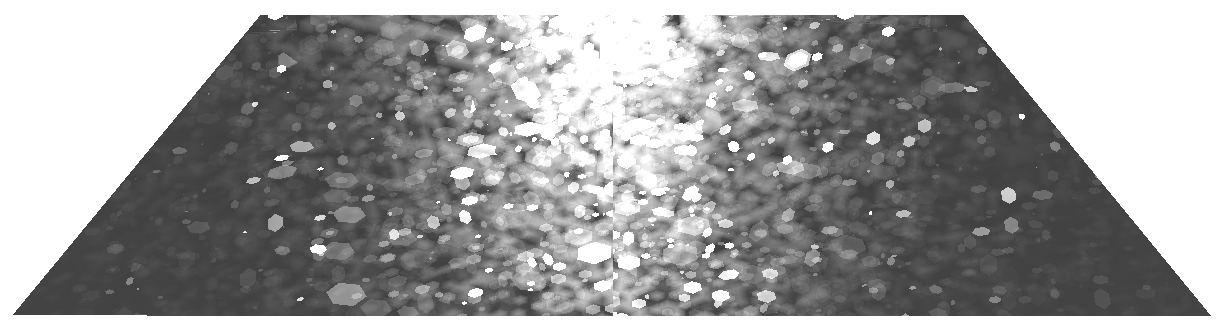
\includegraphics[width=0.5\linewidth]{artifact/distributedsurface.png}
        \caption{Utilizing distributed binomial blending in the surface domain increases the artifact visibility.}
    \end{subfigure}
    \begin{subfigure}{1\linewidth}
        \centering
        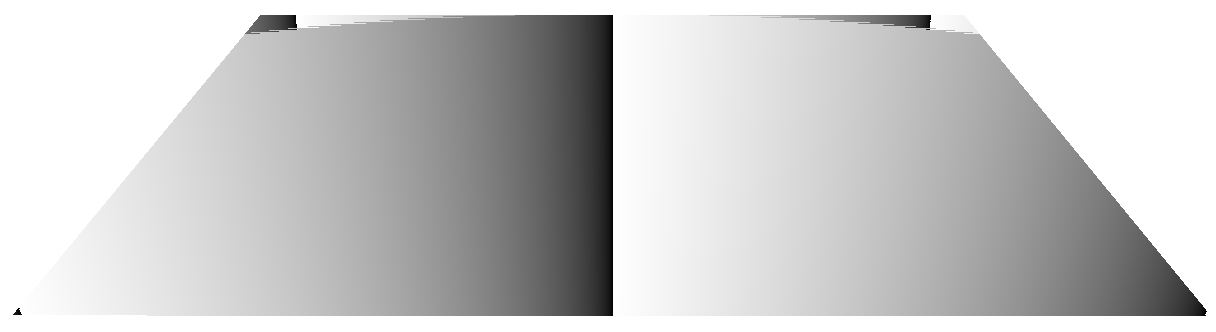
\includegraphics[width=0.5\linewidth]{artifact/thetaweight.png}
        \caption{Visualization of the linear weight in the orientation dimension $\phi$ inside heptahedral cells.}
    \end{subfigure}
    \begin{subfigure}{1\linewidth}
        \centering
        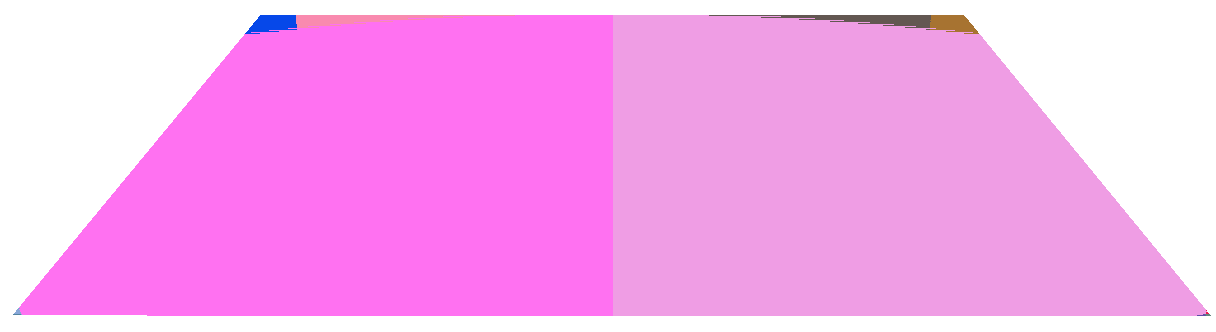
\includegraphics[width=0.5\linewidth]{artifact/heptagrid.png}
        \caption{Individual heptahedral footprint grid cells visualized with hash colors.}
    \end{subfigure}
    \begin{subfigure}{1\linewidth}
        \centering
        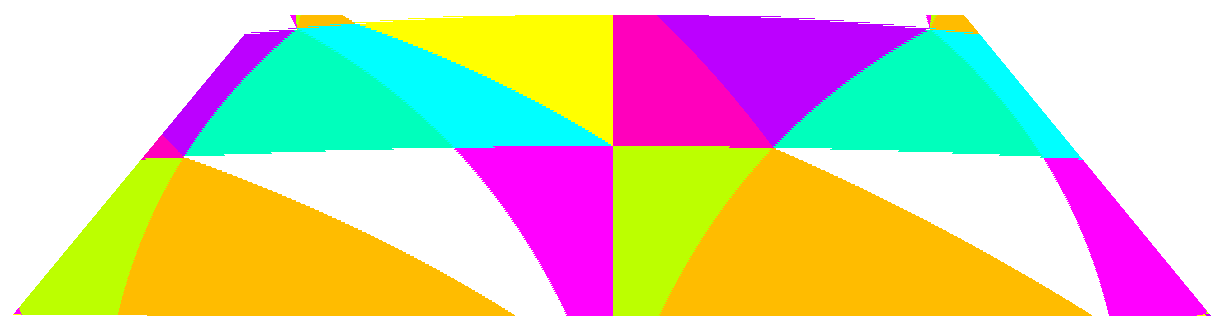
\includegraphics[width=0.5\linewidth]{artifact/tetragrid.png}
        \caption{Branches in tetrahedralization process visualized with colors.}
    \end{subfigure}
    \caption{Images (a) and (b) show a visual artifact occur in the middle. This is exactly where two tetrahedral footprint grid cells touch (e) as the heptahedral grid (d) is divided along the orientation dimension $\phi$ (c). Thus, the artifacts probably occur because of issues with the angular discretization.\label{fig:artifact}}
\end{figure}